\scanpage{134}
% archive sheet number: 133
$\deleted{\unsure{A_1(\mathrm{Si})|A_1(S_i)}}$

\[\left\{\begin{aligned}
&\text{diagrammes } A_2\simeq\text{triangle ponctué \deleted{\unsure{avec}}}\\
&\text{cat des graphes cubiques avec diagramme }A_2\approxeq\text{ catégorie des}\\
&\text{ensembles de cardinal 8 munis d'une involution ss pt}\\
&\text{fixe}\simeq\text{catégorie des 4-cubes}\simeq\text{catégorie des torseurs}\\
&\text{sous }\unsure{\mathfrak S|\mathcal S|\mathcal G}_4.\deleted{\mathbb Z}(\pm1)^4\simeq W_{B_4}\quad\text{(groupe de Weyl de }SO(9))
\end{aligned}\right.\]

\margin{\unsure{détermine|dilemme} pt, triangle -- pas bibase ni \unsure{tripaire|tripode}}
\figure{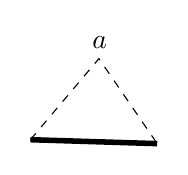
\begin{tikzpicture}
\draw[dashed] (0,0)--(.87,1.03)--(1.61,-.05);\draw[line width=2pt] (0,0)--(1.61,-.05);\node[above] at (.88,1.03){$a$};
\end{tikzpicture}}

\[\left\{\begin{aligned}
&\text{diagrammes }A_3\\
&\simeq\text{ doublet + élément de la demi-étoile associé}\\
&\simeq\text{ bibase \inserted{$B$} + él. marqué de }I=B/\sigma_B+2^{\text{ième}}\ \text{él. marqué}\\
&(\zeta_1,\lambda_{12},\zeta_1^*)\quad\text{él. typiques}\\
&\text{Cat. des graphes cubiques avec diagramme }A_2\approxeq\\
&\text{\deleted{cat des couples}}\ (\mathrm{Ens})_2\times(\mathrm{Ens})_4
\end{aligned}\right.\]

\diagram{\begin{tikzcd}[ampersand replacement=\&,column sep=large]
\zeta_1\arrow[r,no head]\&\underset{\bullet}{\lambda_{12}}\arrow[r,no head]\&\zeta_1^*
\end{tikzcd}}
\margin{détermine pt, bibase, pas triangle ni tripaire}
\figure{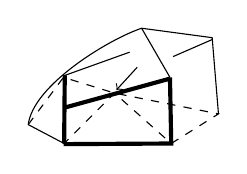
\begin{tikzpicture}[scale=.8]
\draw (0,.45).. controls (.08,1.08) and (1.27,1.8)..(1.8,1.98)--(2.92,1.83)--(3.02,.62);
\draw (2.92,1.8)--(2.3,1.53) (1.8,1.98)--(2.25,1.2) (.55,1.22)--(1.61,1.60) (0,.45)--(.57,.15);
\draw[line width=1.5pt] (.57,.15)--(.58,1.23) (.56,.14)--(2.27,.15)--(2.25,1.2) (.58,.72)--(2.25,1.18);
\draw[dashed] (0,.45)--(.56,1.2)--(1.37,.95)--(3.02,.62)--(2.27,.15)--(1.37,.95)--(.57,.15);
\draw[->] (1.73,1.36)--(1.4,1.00);
\end{tikzpicture}}

\[\left\{\begin{aligned}
&\text{diagrammes } A_4\\
&\simeq\text{pavé + triade et triangle (sécants)}\\
&\deleted{\unsure{\simeq}}\ \simeq\text{hexagone \inserted{dans pavé} + côté}\\
&\approxeq(\mathrm{Ens})_2\times(\mathrm{Ens})_3
\end{aligned}\right.\]
\figure{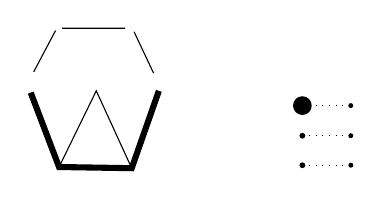
\begin{tikzpicture}[scale=.75]
\draw (0,1.23)--(.37,1.93) (.48,1.97)--(1.55,1.97) (1.7,1.91)--(2.03,1.21);
\draw[line width=2.2pt] (-.05,.88)--(.43,-.38)--(1.66,-.4)--(2.12,.91);
\draw (.43,-.38)--(1.06,.91)--(1.66,-.4);
\foreach \y in {.66,.15,-.35}{\fill (4.55,\y) circle (1.4pt) (5.37,\y) circle(1.2pt);\draw[dotted] (4.55,\y)--(5.37,\y);}
\fill (4.55,.66) circle(4.5pt);
\end{tikzpicture}}

\[\left\{\begin{aligned}
&\text{diagramme }A_5\simeq(\text{\deleted{pavé}\inserted{carré} ponctué})\\
&\hspace{5em}\simeq\text{\deleted{\unsure{carré}}\inserted{hex. ponctué}}\\
&\hspace{5em}\simeq\text{triade épinglée}\\
&\approxeq\mathrm{Ens}_{2\deleted{\unsure{,4}}}\times\mathrm{Ens}_3
\end{aligned}\right.\]
\figure{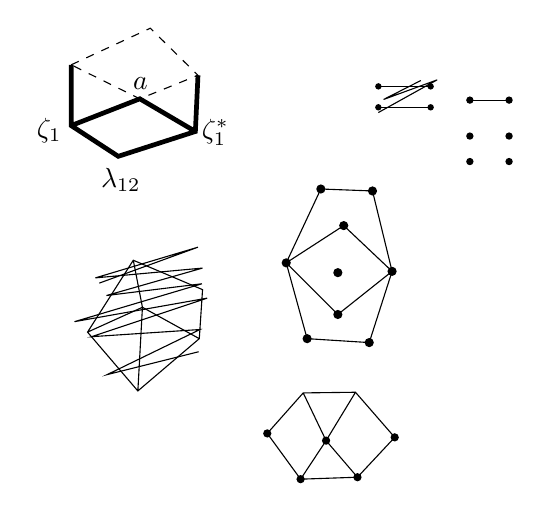
\begin{tikzpicture}[scale=.83]
\draw[line width=1.7pt] (0,1.83)--(0,.9)--(.72,.43)--(1.9,.81)--(1.94,1.67) (0,.9)--(1.05,1.31)--(1.9,.81);
\draw[dashed] (0,1.83)--(1.21,2.39)--(1.94,1.67)--(1.05,1.31)--(0,1.83);
\node[above] at (1.06,1.3){$a$};\node[left] at (0,.82){$\zeta_1$};\node[right] at (1.85,.8){$\zeta_1^*$};\node[below] at (.76,.4){$\deleted{\unsure{\lambda_{12}}}$};
\begin{scope}[xshift=4.7cm,yshift=1.18cm]
\foreach \y in {0,.32}{\draw (0,\y)--(.8,\y);\fill (0,\y) circle(1.4pt) (.8,\y) circle(1.4pt);}
\draw (0,-.08)--(.9,.42)--(.08,.12)--(.65,.41);
\draw (1.4,.11)--(2,.11);\foreach \x in {1.4,2}{\foreach \y in {.11,-.44,-.83}{\fill (\x,\y) circle(1.6pt);}}
\end{scope}
\begin{scope}[xshift=.25cm,yshift=-2.56cm]
\draw (0,.3)--(.7,1.4)--(1.76,.95)--(1.71,.2)--(.77,-.6)--cycle (0,.3)--(.84,.68)--(1.71,.2) (.77,-.6)--(.84,.68)--(.7,1.4);
\draw (.18,1.05)--(1.69,1.6)--(.12,1.13)--(1.76,1.28)--(.29,.86)--(1.75,1.04)--(-.2,.46)--(1.83,.82)--(.06,.23)--(1.72,.34)--(.3,-.35)--(1.7,.0);
\end{scope}
\begin{scope}[xshift=3.29cm,yshift=-1.5cm]
\draw (0,.3)--(.53,1.43)--(1.32,1.40)--(1.62,.17)--(1.27,-.92)--(.32,-.86)--cycle;
\draw (0,.3)--(.88,.87)--(1.62,.17)--(.79,-.49)--cycle;
\foreach \x/\y in {0/.3,.53/1.43,1.32/1.4,1.62/.17,1.27/-.92,.32/-.86,.88/.87,.79/-.49,.79/.15}{\fill (\x,\y) circle(2pt);}
\end{scope}
\begin{scope}[xshift=3cm,yshift=-4.16cm]
\draw (0,.35)--(.55,.97)--(1.35,.98)--(1.95,.29)--(1.38,-.32)--(.51,-.35)--cycle (.55,.97)--(.9,.24)--(1.38,-.32) (.51,-.35)--(.9,.24)--(1.35,.98);
\foreach \x/\y in {0/.35,.9/.24,1.95/.29,.51/-.35,1.38/-.32}{\fill (\x,\y) circle(1.8pt);}
\end{scope}
\end{tikzpicture}}
